%% Philipp G Freimann Juli 2019 für die BBW
%% Phi BBW-Vorlage für Arbeitsblätter (LaTeX)
%% 2019 - 08 - 18

%% %% %% %%
\documentclass[twoside,12pt,a4paper]{article}%%
\usepackage[paper=a4paper,margin=17mm]{geometry}%%


%% Zentralisiert
%%\usepackage{german} %% Macht Probleme mit grafiken
\usepackage{mciteplus}

\usepackage[dvipsnames,table]{xcolor}

\usepackage{pgfplotstable}
\usepackage{tikz}
\usepackage{tkz-euclide} %% Grid

\usepackage{amsthm}
\usepackage{amsfonts} %% Zahlmengen Z, R, ...


%% THEOREMS?
\usepackage{tcolorbox}
\tcbuselibrary{theorems}
\tcbuselibrary{skins}


\usepackage{fancyhdr}
\usepackage{ngerman}
\usepackage[utf8]{inputenc}


%%\usepackage[dvips]{graphicx}

\usepackage{supertabular}
\usepackage{makeidx}  
\usepackage{ifthen} 

\usepackage{multirow}
\usepackage{listings}

%%\usepackage{color,fancyvrb,fancybox}
\usepackage{multicol}
\usepackage{lastpage}
%%\usepackage{listings}
\usepackage{pstricks}

%% bold typewriter font:
\usepackage[T1]{fontenc}
\usepackage{lmodern}

\usepackage{enumitem}
%\usepackage{enumerate}

\usepackage{float}

\usepackage{titlesec}
\usepackage{textcomp}

%% Kuchendiagramme
%%\usepackage{datapie}

%% für Aufgaben Hervorhebung
%%\usepackage[most]{tcolorbox}
%%\usepackage[standard,framed]{ntheorem}
\usepackage{framed}
\usepackage{mdframed}

%%%%%%%%%%%%%%%%%%%%
%%\usepackage[most]{tcolorbox}

\usepackage[tocindentauto]{tocstyle}

%% für accentset wedge:
\usepackage{accents}

%% Würfel
\usepackage{epsdice}

%% Einbinden von GeoGebra Bildchen:
\usetikzlibrary{shapes.geometric}
\usetikzlibrary{arrows}
\newcommand{\degre}{\ensuremath{^\circ}}

%% Hyperlinks
\usepackage{hyperref}

\hypersetup{
    colorlinks=true,
    linkcolor=blue,
    filecolor=magenta,      
    urlcolor=cyan,
    bookmarks=true,
}

%% bugtracker (part of pgfplots) should be loaded AFTER "hyperref"
%% See: https://texblog.net/hyperref/ AND https://tex.stackexchange.com/questions/16268/warning-with-footnotes-namehfootnote-xx-has-been-referenced-but-does-not-exi
\usepackage{pgfplots}
\pgfplotsset{width=10cm,compat=1.9}

%%\usepackage{fourier}  %% eg overarc (Bogenmaß)

%%%%%%%%%%%%%%%%% L A Y O U T  %%%%%%%%%%%%%%%%%%%%%%%%%%%%
%% 2020-12-27 ph. g. freimann @ bbw.ch
%%

\fancyhf{}%%

\pagestyle{fancy}%%

\renewcommand{\sectionmark}[1]{%%
  \markboth{\thesection{} \ #1}{}%%
}%%

\renewcommand{\subsectionmark}[1]{%%
  \markright{\thesubsection \ #1}%%
}%%

%% Achtung: chaptermark nur im BOOK-Style

\renewcommand{\footrulewidth}{0.4pt}

\parskip4pt
\parindent0pt

\topmargin-2.0cm
\textheight24.4cm

\renewcommand{\arraystretch}{1}%%


\newenvironment{bbwFillInTabular}{%%
%% BEGIN PART:
\renewcommand{\arraystretch}{2.1}
\begin{tabular}%%
}%% END PART:
{\end{tabular}
\renewcommand{\arraystretch}{1}%%
}%% END Environment bbwFillInTabular

%%%%%%%%%%%%%%%%%%%%%%%%%%%%%%%%%%%%%%%%%%%%%%%%%%%%%%%%%%
%%%%%%%%%%%%%%%%%% M A K R O S %%%%%%%%%%%%%%%%%%%%%%%%%%%
%%%%%%%%%%%%%%%%%%%%%%%%%%%%%%%%%%%%%%%%%%%%%%%%%%%%%%%%%%

%%%%%%%%%%%%%%%%%%%%%%%% g e n e r e l l e   M a k r o s %%%%%%%%%%%%%%%%%%%%%%%

%% Info vorab bei \newcommand
%% \newcommand{ - Kommandos können in den Parametern auch Leerzeilen
%%     enthalten
%% \newcommand*{ - Kommandos, also mit *, können jedoch in den
%%    Argumenten KEINE \par (sprich Leerzeilen} enthalten

%% 2019-07-26
%% phi@freimann.eu
%% Makros for BBW-Tex Documents
\usepackage{inputs/bbwColors}

%%%%%%%%%%%%%%%%%% I N C L U D E S   &   I N D E X  %%%%%
\graphicspath{{../img/}}
\graphicspath{{./img/}}

\newcommand*\bbwGraphicRaise[3]{\raisebox{#1}{\includegraphics[width=#2]{#3}}}%%
\newcommand*\bbwGraphic[2]{\bbwGraphicRaise{-5mm}{#1}{#2}}%%
\newcommand*\bbwCenterGraphicRaise[3]{\begin{center}\bbwGraphicRaise{#1}{#2}{#3}\end{center}}
\newcommand*\bbwCenterGraphic[2]{\bbwCenterGraphicRaise{-5mm}{#1}{#2}}%%


%% All in one Skript
\newif\ifisALLINONE
\isALLINONEfalse

%% Blended Learning
%% Insb. MatheNinja Links. Diese sind jedoch in einem anderen Kurs!
\newif\ifisBLENDED
\isBLENDEDfalse


%%%%%%%%% TRAINER Version vs. Schülerversion %%%%%%%%%%%%%
%% Bem. Kein *-Kommando, da die TRAINER-Blöcke auch leerzeilne (\par)
%% enthaltne können
\newcommand\TRAINER[1]{%%
{%%
\ifisTRAINER{\color{BlueGreen}{#1}}%%
\fi%%
}}%%  

\newcommand\TALS[1]{%
{%%
\ifisTALS{#1}%%
\fi%%
}}%

\newcommand\GESO[1]{%
{%%
\ifisGESO{#1}%%
\fi%%
}}%    

\newcommand\BLENDED[1]{%
{%%
\ifisBLENDED{#1}%%
\fi%%
}}%    

\newcommand{\noTRAINER}[1]{{\ifisTRAINER{}\else{#1}\fi}{}}%%



%%\makeatletter
%% Je nach Umgebung "environment" wird das mmPapier breiter oder
%% schmaler
%% bei itemize sollen 16.4 und bei definiton-Boxen 16.8 mm genommen
%% werden.


\usepackage{inputs/mmPapierbreiteSty}


%% Trainer "no" Dotfill
%% If no Trainer: Dotfill
\newcommand*{\TNDF}[1]{\TRAINER{#1}\noTRAINER{\dotfill{}}}%%

\newcommand*{\leserluft}{\vspace{2mm}}

%% Notiz felder 
%% Anwendung:
%% \noteField{10}  
%%  --> Notizfeld mit 10 Leerzeilen
\newcounter{DFCounter}


%%Häuschenpapier
\newcommand{\mmPapierZwei}[2]{\begin{tikzpicture}
%%  \draw[step=4mm,bbwMMFarbe,ultra thin]
%%  \draw[step=4mm,bbwMMFarbe,thick]
  \draw[step=4mm,bbwMMFarbe,line width=0.02mm]
  (0, 0) grid ({#2}, {#1});
\end{tikzpicture}}%%


%% millimeterPapier füllen bis Ende Seite
\newcommand{\mmPapierBisEndeSeite}{

\begin{tikzpicture}

\newdimen\spaceleftOnPage
\spaceleftOnPage=\dimexpr\textheight-\pagetotal-14pt\relax

\pgfmathsetmacro{\gridWidth}{\textwidth        - mod(\textwidth,      4mm)      }
\pgfmathsetmacro{\gridHeight}{\spaceleftOnPage - mod(\spaceleftOnPage,4mm) - 4mm}

\draw [step=4mm,bbwMMFarbe,line width=0.02mm] (0,0) grid (\gridWidth pt,\gridHeight pt);
\end{tikzpicture}%%
\newpage%%
}%% END Makro mmPapieBisEndeSeite


%% Standardbreite für Arbeitsblätter und das Theorieheft
%% Wird in bbwPruefung.sty überschrieben, da dort schmaler
\def\defaultTextBreite{17.6}
\def\unitCMWhatElse{cm}%% wird als Breitenangabe für den nächsten command verwendet

%% Verwendung: \bbwCenterGraphic{\defaultTextBreite}{«img url»}
\def\defaultTextBreiteCM{\defaultTextBreite\unitCMWhatElse}
\newcommand{\mmPapier}[1]{\mmPapierZwei{#1}{\defaultTextBreite}}


%% Notizen Berechungen auf Prüfungsblättern
\newcommand{\platzFuerBerechnungen}[1]{\noTRAINER{

Notizen / Berechnungen:

\mmPapier{#1}}}%% end platzFuerBerechnungen

\newcommand{\platzFuerBerechnungenBisEndeSeite}[1]{\noTRAINER{

Notizen / Berechnungen:

\mmPapierBisEndeSeite}}%% end platzFuerBerechnungen



\newcommand{\platzFuerBerechnungenOhneText}[1]{\noTRAINER{

\mmPapier{#1}}}

%% Die Abkürzung z.\,B. von «Zum Beispiel» hat einen verkleinerten Abstand.
\newcommand*\zB{%
z.\,B.
}

%%
%% Auf der Titelseite steht entweder GESO oder TALS.
%% Dies wird gleich mit der Fußnote angegeben.
%% Dieses Kommando sollte im Kommando «\untertitel» eingesetzt werden.
%%
\newcommand*\ausrichtungAufTitelseite{%
\ifisTALS{TALS\noTRAINER{\footnote{TALS «Technik, Architektur und Life Sciences
(Laboranten)»: Ausrichtung technisches Profil}}}%%
\fi%%
\ifisGESO{GESO\noTRAINER{\footnote{GESO: Ausrichtung \textbf{Ge}sundheit und \textbf{So}ziales}}}%%
\fi}%%

%%%%%%%%%%%%%%%%%%%%%% B B W - M a t h e   F a r b c o d e s  %%%%%%%%%%%%%%%%%%%%%%%%%%%%%%555

\newcommand{\rezeptFarbe}{rezeptFarbe}
\newcommand{\definitionFarbe}{definitionFarbe}
\newcommand{\gesetzFarbe}{gesetzFarbe}
\newcommand{\beispielFarbe}{beispielFarbe}
\newcommand{\bemerkungFarbe}{bemerkungFarbe}

%% Falls gewünscht übersteuren
%  \definecolor{xyz}{HTML}{eeff66}
%  \renewcommand{\beispielFarbe}{xyz}
%

%% Theorem-Styles
\newcommand\theoremlayoutdefinition[4]{\newtcbtheorem[number within=section]{#1}{#2}%
   {theorem style=plain,enhanced,colframe=#3!20!white,colback=#3!20!white,
     coltitle=#3!60!black,fonttitle=\upshape\bfseries,
     %%fontupper=\itshape,
    %%drop fuzzy shadow=blue!50!black!50!white,
    terminator sign={:},
    borderline north={0.5mm}{0pt}{#3}, borderline south={0.5mm}{0pt}{#3}
}{#4}}



%% Farben für rezept, definition und gesetz von Marthale übernommen.
%% Verwendung mit * unterbindet die Nummerierung \begin{gesetz*}{Blah}{xy} ...\end {gesetz*}
\theoremlayoutdefinition{rezept}{Rezept}{\rezeptFarbe}{R}
\theoremlayoutdefinition{definition}{Definition}{\definitionFarbe}{D}
\theoremlayoutdefinition{gesetz}{Gesetz}{\gesetzFarbe}{G}%% was green
\theoremlayoutdefinition{beispiel}{Beispiel}{\beispielFarbe}{B}
\theoremlayoutdefinition{bemerkung}{Bemerkung}{\bemerkungFarbe}{M}

%%
%% Force a blank page, when \newpage does not work
%%
\def\blankpage{%
	\clearpage%
	\null%
	\clearpage}%%

\newcommand{\Lueckentext}[1]{\,\,\noTRAINER{\dotfill}\TRAINER{#1}}


\newcommand{\LoesungsRaumCM}[2]{\,\,\noTRAINER{\underline{\hspace{#1}}}\TRAINER{#2}}

\newcommand{\LoesungsRaum}[1]{\LoesungsRaumCM{30mm}{#1}}
\newcommand{\LoesungsRaumKurz}[1]{\LoesungsRaumCM{15mm}{#1}}
\newcommand{\LoesungsRaumLang}[1]{\LoesungsRaumCM{45mm}{#1}}


%% TI nSpire
\def\tinspire{\texttt{TI-nSpire}}

%% TI 30 Pro Mathprint Button Images
\def\tiprobuttonbreite{10mm}
\def\nspirebuttonbreite{8.6mm}

%%\def\sec{\raisebox{-2mm}{\includegraphics[width=\buttonbreite{}]{img/tiprobuttonimages/2nd.png}}}
\newcommand{\tiprobutton}[1]{\raisebox{-2mm}{\mbox{\,\includegraphics[width=\tiprobuttonbreite{}]{img/tiprobuttonimages/#1.png}\,}}}

\newcommand{\nspirebutton}[1]{\raisebox{-2mm}{\mbox{\,\includegraphics[width=\nspirebuttonbreite{}]{img/nspirebuttonimages/#1.png}\,}}}

%% Counter  für Aufgaben
%% Bei jedem Part wird die Aufgabennummer zurückgesetz auf 1
\newcommand{\bbwPartID}{AA1}
\newcommand{\bbwAufgabenBlockID}{}
\newcounter{bbwAufgabenNummerCounter}[part]
\setcounter{bbwAufgabenNummerCounter}{1}
\newcommand{\bbwAufgabenNummer}{\arabic{bbwAufgabenNummerCounter}}
\newcommand{\nextBbwAufgabenNummer}{\stepcounter{bbwAufgabenNummerCounter}}
\newcommand{\aufgSubLabel}{{\color{blue}\bbwAufgabenNummer. \alph*)}}

%% Benutze außerhalb der bbwAufgabenblöcke folgendes Kommando, um an die
%% nächste Aufgabennummer zu kommen. Dies z. B. wenn ein längerer Text vor der Aufgabe steht,
%% der auch schon diese Bezeichnung erhalten sollte
\newcommand{\bbwActAufgabenNr}{{\color{blue}\bbwAufgabenNummer. {\small[\bbwAufgabenBlockID]}}}


\newenvironment{bbwAufgabenBlock}{%% Begin environment Part:

\bbwActAufgabenNr{}
%%{\color{blue}\bbwAufgabenNummer. {\small[\bbwAufgabenBlockID]}}
\begin{enumerate}[label=\aufgSubLabel]
}%% Ende der Präambel
{%% END Part:
\end{enumerate}
\nextBbwAufgabenNummer
}%% END environment bbwAufgabenBlock

%%%%%%%%%%%%%%%%%%%%%%%%%%%%

%% Weblinks und Mathe Ninja Links

\newcommand{\weblink}[2]{\href{#2}{#1}}

\newcommand{\olatBBWLogo}{
\includegraphics[width=15mm]{logos/traube.pdf}}%%
\newcommand{\externerLinkEPS}{
\includegraphics[width=15mm]{logos/extLink.pdf}}%%
\newcommand{\youtubeLogo}{\includegraphics[width=15mm]{logos/youtube.png}}%%


%%
%% #1: Text
%% #2: URL
%% #3: Aufgabennummern
%% #4: optional weitere Logos oder leer lassen {}
\newcommand{\externalLink}[4]{%%
\begin{tabular}{|lp{111mm}|}\hline%%
\multicolumn{2}{|p{172mm}|}{\cellcolor{aufgabenFarbe}#3}\\
\weblink{\raisebox{-5mm}{\externerLinkEPS{}}}{#2} {#4}  & \weblink{#1}{#2}\\\hline
\multicolumn{2}{|p{172mm}|}{\weblink{#2}{#2}}\\\hline
\end{tabular}%%
\vspace{1mm}
}%% END Command externalLink

%% #1: URL
%% #2: Text
\newcommand{\youtubeLink}[2]{%%
\externalLink{#2}{#1}{Youtube}{\raisebox{-5mm}{\youtubeLogo{}}}
}%%

%%
%% #1: Typ-Logo (eg. LOGO auf MatheNinja)
%% #2: Typ-Name (eg «Mathe Ninja»
%% #3: URL
%% #4: Aufgaben Name
\newcommand{\olatLink}[4]{%%
\begin{tabular}{|lp{111mm}|}\hline%%
\multicolumn{2}{|p{172mm}|}{\cellcolor{aufgabenFarbe}#4}\\
\weblink{\raisebox{-5mm}{\externerLinkEPS{}}}{#3} \weblink{\raisebox{-5mm}{\olatBBWLogo}}{#3} \weblink{#1}{#3}& \weblink{#2}{#3}\\\hline
\end{tabular}%%
\vspace{1mm}
}%% END Command olatLink


%\newcommand{\olatLOGOLink}[3]{%%
%\begin{tabular}{|lp{111mm}|}\hline%%
%\weblink{\raisebox{-5mm}{\olatBBWLogo{}}}{#2} & \weblink{#1}{#2}\\
%\multicolumn{2}{|p{172mm}|}{\cellcolor{aufgabenFarbe}#3}\\\hline
%\end{tabular}%%
%}%% END Command olatLOGOLink

%% Use:
%% \olatLinkArbeitsblatt{Kapitel/Arbeitsblattname «[ID]»}{«URL»}{Aufgabennummern}
\newcommand{\olatLinkArbeitsblatt}[3]{\olatLink{\raisebox{-6mm}{
\includegraphics[width=12mm]{logos/seite.pdf}}}{Arbeitsblatt: #1}{#2}{#3}}%%

%% #1: Text
%% #2: URL
\newcommand{\olatLinkPruefung}[2]{\olatLink{\raisebox{-6mm}{
\includegraphics[width=15mm]{logos/test.pdf}}}{Online Test}{#2}{#1}}%%


%%
%% use:
%% \matheNinjaLink{Beschreibung}{URL}
\newcommand{\matheNinjaLink}[2]{\olatLink{\raisebox{-6mm}{\includegraphics[width=17mm]{img/matheninja/matheninja.jpg}}}{Mathe Ninja!}{#2}{#1}}%%


%% Use
%% \olatLinkGESOKompendium{Kapitel}{Seite/Seiteff}{Aufgabe(n)}
\newcommand{\olatLinkGESOKompendium}[3]{%%
\GESO{%%
\olatLink{{\Huge K}}{Kompendium}{https://olat.bbw.ch/auth/RepositoryEntry/572162163/CourseNode/106029172671728}{Kapitel #1; Seite #2; Aufg. #3}%%
}%% END GESO
}%%


%% Use \olatLinkTALSStrukturaufgabenSPF{Kapitel}{Seite/Seiteff}{Aufgabe(n)}
\newcommand{\olatLinkTALSStrukturaufgabenSPF}[3]{%%
\TALS{%%
\olatLink{{\Huge S}}{Strukturaufgaben}{https://olat.bbw.ch/auth/RepositoryEntry/572162090/CourseNode/102901174299246}{Kapitel #1; Seite #2; Aufgaben #3}%%
}%% END GESO
}%%

%%\newcommand{\olatLinkTALtfSStrukturaufgabenGLF}[1]{\olatLOGOLink{Strukturaufgaben Grundlagenfach}{https://olat.bbw.ch/auth/RepositoryEntry/572162090/CourseNode/102901174291476}{#1}}


%%\newcommand{\matheNinjaLink}[2]{%%
%%\begin{tabular}{cc}%%
%% \raisebox{-1cm}{\includegraphics[height=2cm]{img/matheninja/turtle.png}}& \href{#2}{MatheNinja: #1}\\%%
%% \end{tabular}%%
%%}%% End Command  \matheNinjaLink



%% AadB = Aufgaben aus dem Buch
%% 1. Parameter: Seitenzahl
%% 2. Parameter: Aufgabennummern.
%% bsp  \TALSAadB{38-39}{101a-101c, 102 und 103}

%%\newcommand*{\maturaAufgaben}[1]{\begin{mdframed}[backgroundcolor=maturaAufgabenFarbe!10]{#1}\end{mdframed}}

\newcommand*{\aadBTxt}{Aufgaben aus dem Buch}


%%
% Generell Aufgaben aus einem Lehrbuch
% #1: cite auf das Lehrbuch (z. B. frommenwiler17alg)
% #2: Seitennummer oder Seitennumerff
% #3: aufgabennummer(n)
\newcommand*{\AadB}[3]{%%
\aufgabenFarbe{\noindent{\aadBTxt \cite{#1}: Seite {#2} Nr. {#3}}}%%
}%%

%%\newcommand*{\AdbBAlgebra}[2]{\AadB{marthaler21alg}{#1}{#2}}%%

\newcommand*{\TALSAadBFWA}[2]{\ifisTALS{\AadB{frommenwiler17alg}{#1}{#2}}\fi}%%
\newcommand*{\TALSAadBMTA}[2]{\ifisTALS{\AadB{marthaler21alg}{#1}{#2}}\fi}%%
\newcommand*{\TALSAadBFWG}[2]{\ifisTALS{\AadB{frommenwiler18geom}{#1}{#2}}\fi}%%
\newcommand*{\TALSAadBMTG}[2]{\ifisTALS{\AadB{marthaler20geom}{#1}{#2}}\fi}%%

%% GESO hat (noch) keine Geometrie
\newcommand*{\GESOAadBMTA}[2]{\ifisGESO{\AadB{marthaler21alg}{#1}{#2}}\fi}%%

\newcommand*{\AadBMTA}[2]{\AadB{marthaler21alg}{#1}{#2}}
\newcommand*{\AadBMTG}[2]{\AadB{marthaler20geom}{#1}{#2}}

%%
% Generell Theorie aus einem Lehrbuch
% #1: cite auf das Lehrbuch (z. B. frommenwiler17alg)
% #2: Seitennummer oder Seitennumerff
% #3: KapitelNummer
\newcommand*{\TadB}[3]{%%
\aufgabenFarbe{\noindent{Theorie \cite{#1}: Seite {#2} Nr. {#3}}}%%
}%%

\newcommand*{\TALSTadBFWA}[2]{\ifisTALS{\TadB{frommenwiler17alg}{#1}{#2}}\fi}%%
\newcommand*{\TALSTadBMTA}[2]{\ifisTALS{\TadB{marthaler21alg}{#1}{#2}}\fi}%%
\newcommand*{\TALSTadBFWG}[2]{\ifisTALS{\TadB{frommenwiler18geom}{#1}{#2}}\fi}%%
\newcommand*{\TALSTadBMTG}[2]{\ifisTALS{\TadB{marthaler20geom}{#1}{#2}}\fi}%%

%% GESO hat (noch) keine Geometrie
\newcommand*{\GESOTadBMTA}[2]{\ifisGESO{\TadB{marthaler21alg}{#1}{#2}}\fi}%%
\newcommand*{\TadBMTA}[2]{\TadB{marthaler21alg}{#1}{#2}}
\newcommand*{\TadBMTG}[2]{\TadB{marthaler20geom}{#1}{#2}}


%% Referenzen auf Labels
%% AllInOne ist wichtig, denn einige Referenzen funkitionieren nicht
%% in den Themen-Skripts, sondern lediglich in den gesamten Jahres-Skripts.
\newcommand*\totalref[1]{\ifisALLINONE{ (s.\kern 0.22em{}Kap. \ref{#1}
    auf Seite \pageref{#1}) }\else{}\fi{}}%%
\newcommand*\totalrefanhang[1]{ (s.\kern 0.22em{}Kap. \ref{#1}
    auf Seite \pageref{#1}) }%%

%% Short version
\newcommand*\totalrefs[1]{\ifisALLINONE{ Kap. \ref{#1} auf Seite
\pageref{#1} }\else{}\fi{}}%%
%%\newcommand*\aufgabenref[1]{(s\kern 0.22em{}Aufg. \ref{#1} auf Seite \pageref{#1})}

%%%%%%%%%%%%%%%%%%%%%%%%%%%%%%%%%%% BBW Makros %%%%%%%%%%%%%%%%%%%%%%%%%%%%%


%% Philipp G Freimann Juli 2019 für die BBW
%% Phi BBW-Vorlage für Mathematische Dokumente (LaTeX)
%% 2019 - 07 - 11
%%%%%%%%%%%%%%%%%%%%%%%%%%% M a t h e   M a k r o s %%%%%%%%%%%%%%%%%%%%%%%%%%%%%5

\usetikzlibrary{arrows.meta}

%% Kleine Symbole über anderen. Z. B. "?" über einem
%% Gleichheitszeichen:
%% Use \ueberMini{=}{?} um ein kleines Fragezeichen über ein
%% Gleichheitsszeichen zu schreiben.
\newcommand{\ueberMini}[2]{ \mathrel{\stackrel{\makebox[0pt]{\mbox{\normalfont\tiny #2}}}{#1}} }

%% Gleichungssystem mit zwei Zeilen und vier Einträgen (je zwei links
%% bzw. rechts).
\def\gleichungZZ#1#2#3#4{%%
  $$\left|
  \begin{array}{rcl}
    {#1} &=& {#2}\\
    {#3} &=& {#4}
    \end{array}\right|$$}%%

\def\gleichungDD#1#2#3#4#5#6{%%
  $$\left|
  \begin{array}{rcl}
    {#1} &=& {#2}\\
    {#3} &=& {#4}\\
    {#5} &=& {#6}\\
    \end{array}\right|$$}%%

%% Entspricht-Symbol
%%\usepackage{accents}
\newcommand{\hatset}[1]{\accentset{\wedge}{#1}}
\newcommand{\entspricht}{\,\,\hatset{=}\,\,}
\newcommand*\mittelwert[1]{\bar{#1}}
\newcommand*\mediantilde[1]{\widetilde{#1}}

%%
%% Graphiken mit tikz: BBW-Mathe-akros
%%
\tikzset{bbwgrid/.style={help lines,color=cyan!18, step=0.5cm}}

\newcommand{\bbwGridPart}[4]{
 % grid:
 \draw[bbwgrid] (#1,#3) grid (#2,#4);

 % axes
 \draw[thick] (#1,0) -- (#2,0);
 \draw[thick] (0,#3) -- (0,#4);
 \foreach \x in {#1, ..., -1}  \draw (\x cm, 2pt) -- (\x cm, -2pt)  node[anchor=north]{$\x$};
 \foreach \x in {1, ..., #2}   \draw (\x cm, 2pt) -- (\x cm, -2pt)  node[anchor=north]{$\x$};
 \foreach \y in {#3, ..., -1}  \draw (-2pt, \y cm) -- (2pt, \y cm)  node[anchor=east]{$\y\,\,$};
 \foreach \y in {1, ..., #4}   \draw (-2pt, \y cm) -- (2pt, \y cm)  node[anchor=east]{$\y\,\,$};
 \draw[->,thick] (#2,0) -- ({#2+0.5},0) node[anchor=west]{$x$};
 \draw[->,thick] (0,#4) -- (0,{#4+0.5}) node[anchor=south]{$y$};
}


%% A function within a Grid (without painting the grid)
%% #1: funciton eg 2*\x  (x has to be backquoted)
%% #2: Domain eg. -1:2.5
%% #3: colour eg red
\newcommand{\bbwFuncC}[3]{\draw[domain=#2,smooth,samples=200,variable=\x,#3] plot ({\x},{#1});
}
%% A function within a Grid (without painting the grid)
\newcommand{\bbwFunc}[2]{\bbwFuncC{#1}{#2}{blue}}

%% Declare a function-plot
%% xmin,xmax,ymin,ymax,fct,domain(x-min, x-max)
%% example: \bbwFunction{-4}{3}{-2}{5}{-\x*\x- \x + 4.5}{-3:2}
\newcommand{\bbwFunction}[6]{\begin{tikzpicture}
\bbwGridPart{#1}{#2}{#3}{#4}
 \bbwFunc{#5}{#6}
%% \draw[domain=#6,smooth,samples=200,variable=\x,blue] plot ({\x},{#5});
\end{tikzpicture}}
%% a whole graph having a coordinate-system #1-#4 and any tizpicture content #5:
\newcommand{\bbwGraph}[5]{\begin{tikzpicture}\bbwGridPart{#1}{#2}{#3}{#4}#5\end{tikzpicture}}

%% Dots and lines:
%% Dot example: \bbwDot{-1,2}{red}{east}{A}
\newcommand{\bbwDot}[4]{\filldraw[color=#2!60, fill=#2!5, thick](#1) circle(0.05) node[anchor=#3]{$#4$};}

%% Line example: \bbwLine{-1,0}{2,3}{red}
\newcommand{\bbwLine}[3]{\draw[thick,color=#3] (#1)--(#2);}

\newcommand{\bbwArrow}[3]{\draw[thick,color=#3,->] (#1)--(#2);}


%% Draw a single letter or small text
% #1: Position eg  4,4
% #2: letter eg f or blah
% #3: colour
\newcommand{\bbwLetter}[3]{\draw[color=#3](#1) node{$#2$};}

%%% ABC-Formel
%% usage \abcd{<a>}{<b>}{<c>}
%% example usage: \abcd{b}{5}{\sqrt{4}}
\newcommand{\abcd}[3]{$\frac{-(#2)\pm\sqrt{(#2)^2 - 4\cdot{}(#1)\cdot{}(#3)}}{2\cdot{}(#1)}$}



%% Trigonometrische Koordinatensysteme
%% Alle heißen "trigsysS" wobei da S einer der folgenden Sub-Systeme
%% bezeichnet:
%%  A  phi von  0 ... 360
%%     y   von -3 ...   3
%%
%%  B  phi von  0 ... 360
%%     y   von -1 ...   1
%%
%%  C  phi von  -270 ... 450
%%     y   von    -2 ...   2
%%
%%  D  phi von  -270 ... 450
%%     y   von    -1 ...   1
%%

\newcommand{\trigsysA}{
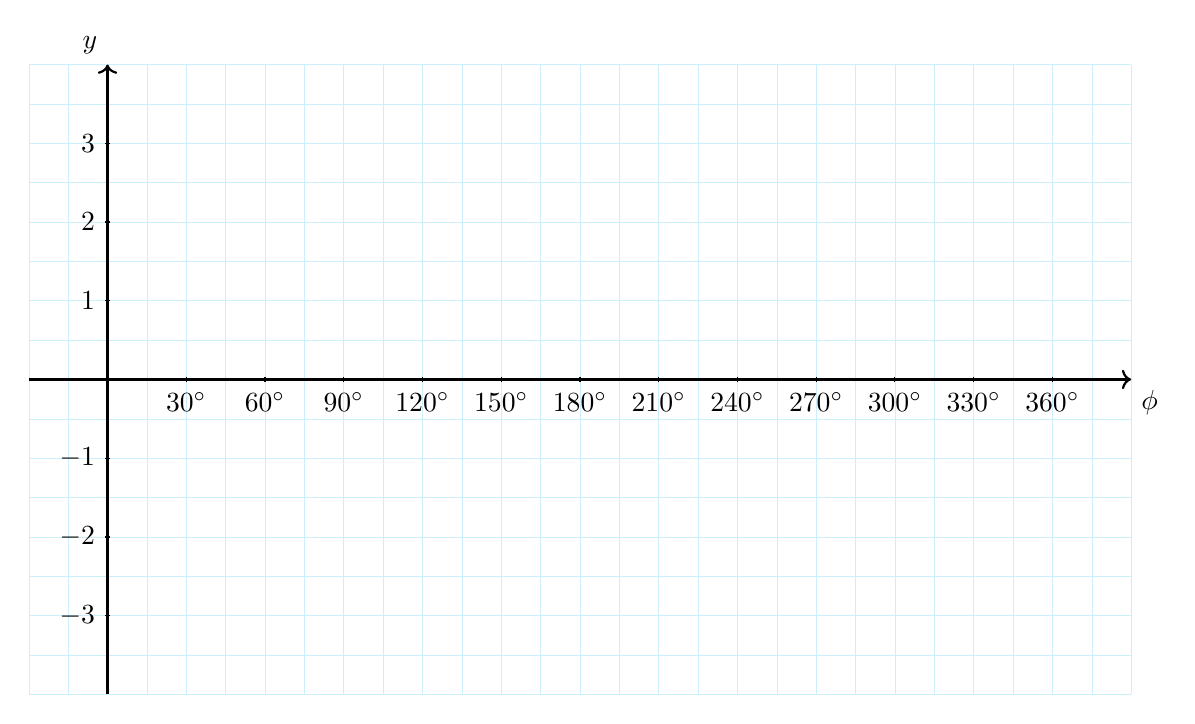
\begin{tikzpicture}
\draw[step = 0.5 cm, cyan!20 , very thin] (-1, -4) grid ( 13, 4);
\draw[thick, ->] (-1,0) -- (13,0) node[anchor = north west] {$\phi$};
\draw[thick, ->] (0,-4) -- (0,4) node[anchor = south east] {$y$};

\foreach \x [evaluate=\x as \degree using int(\x*30)] in {1,...,12}{ 
   \draw (\x cm, 1pt) -- (\x cm, -1pt) node[anchor = north] {$\degree^\circ$};
   }
\foreach \y in {-3,-2,-1,1,2,3}
   \draw (1pt, \y cm) -- (-1pt, \y cm) node[anchor = east] {$\y$};
\end{tikzpicture}}%% END Definition

\newcommand{\trigsysB}{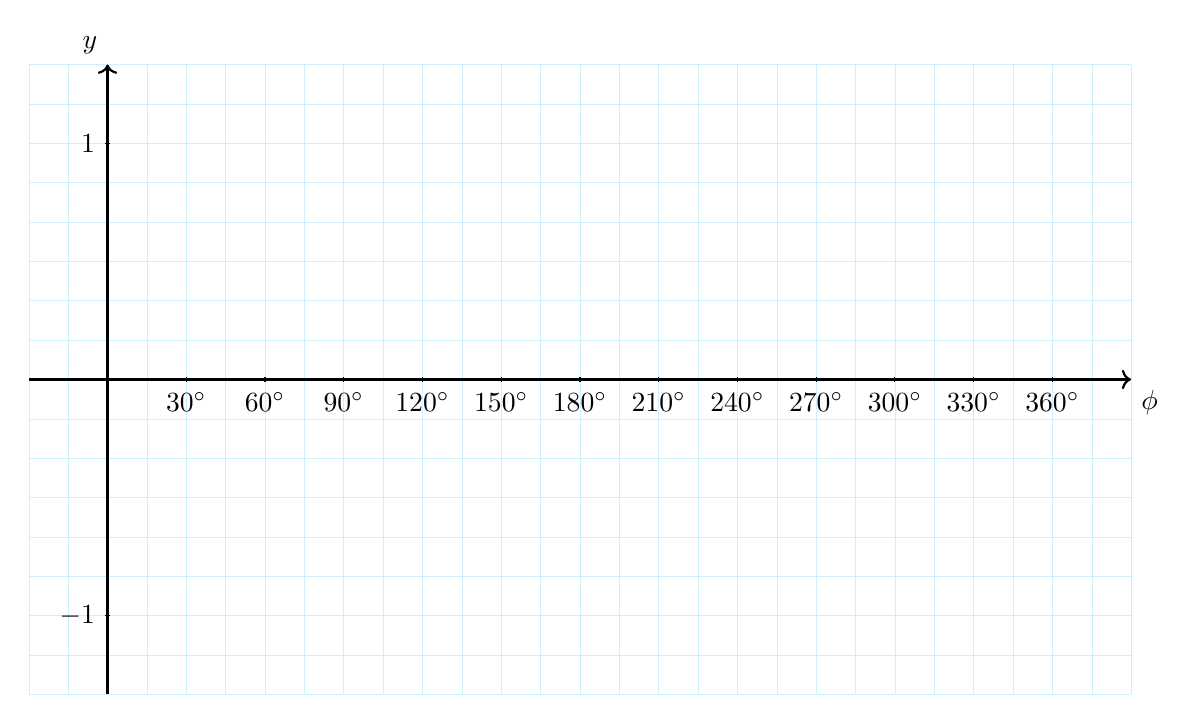
\begin{tikzpicture}\draw[step = 0.5 cm, cyan!20 , very thin] (-1, -4) grid ( 13, 4);
\draw[thick, ->] (-1,0) -- (13,0) node[anchor = north west] {$\phi$};
\draw[thick, ->] (0,-4) -- (0,4) node[anchor = south east] {$y$};

\foreach \x [evaluate=\x as \degree using int(\x*30)] in {1,...,12}{ 
   \draw (\x cm, 1pt) -- (\x cm, -1pt) node[anchor = north] {$\degree^\circ$};
   }
\foreach \y in {-1,1}
   \draw (1pt, \y *3cm) -- (-1pt, \y *3cm) node[anchor = east] {$\y$};

\end{tikzpicture}}%% END Definition

\newcommand{\trigsysC}{
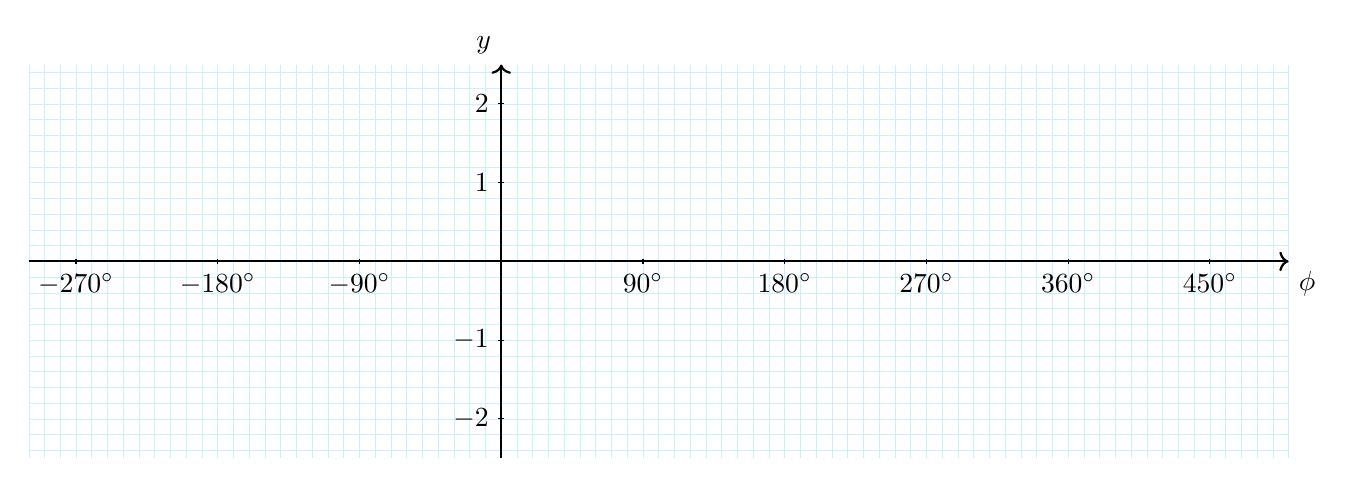
\begin{tikzpicture}
\draw[step = 0.2 cm, very thin, cyan!20] (-6, -2.5) grid ( 10, 2.5);
\draw[thick, ->] (-6,0) -- (10,0) node[anchor = north west] {$\phi$};
\draw[thick, ->] (0,-2.5) -- (0,2.5) node[anchor = south east] {$y$};

\foreach \x [evaluate=\x as \degree using int(\x*90)] in {-3,-2,-1,1,2,3,4,5}{ 
   \draw (\x *18mm, 1pt) -- (\x * 18mm, -1pt) node[anchor = north] {$\degree^\circ$};
   }
   
\foreach \y in {-2,-1,1,2}
   \draw (1pt, \y cm) -- (-1pt, \y cm) node[anchor = east] {$\y$};
\end{tikzpicture}}%% END Definition

\newcommand{\trigsysD}{
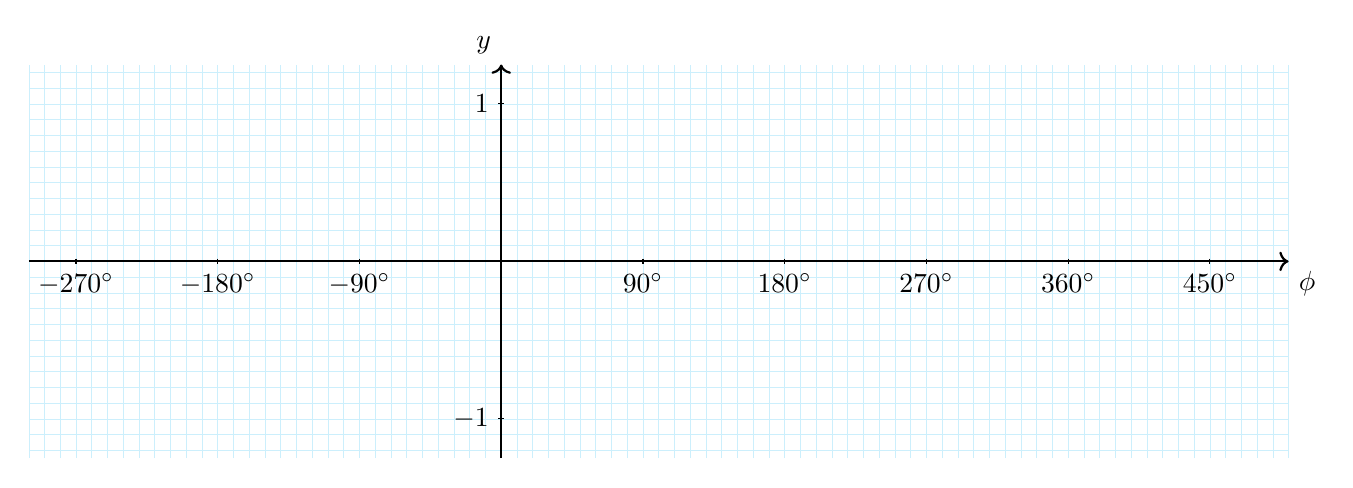
\begin{tikzpicture}
\draw[step = 0.2 cm, very thin, cyan!20] (-6, -2.5) grid ( 10, 2.5);
\draw[thick, ->] (-6,0) -- (10,0) node[anchor = north west] {$\phi$};
\draw[thick, ->] (0,-2.5) -- (0,2.5) node[anchor = south east] {$y$};

\foreach \x [evaluate=\x as \degree using int(\x*90)] in {-3,-2,-1,1,2,3,4,5}{ 
   \draw (\x *18mm, 1pt) -- (\x * 18mm, -1pt) node[anchor = north] {$\degree^\circ$};
   }
   
\foreach \y in {-1,1}
   \draw (1pt, \y *2cm) -- (-1pt, \y *2cm) node[anchor = east] {$\y$};
\end{tikzpicture}}%% END Definition


\newcommand{\trigsysDsin}{
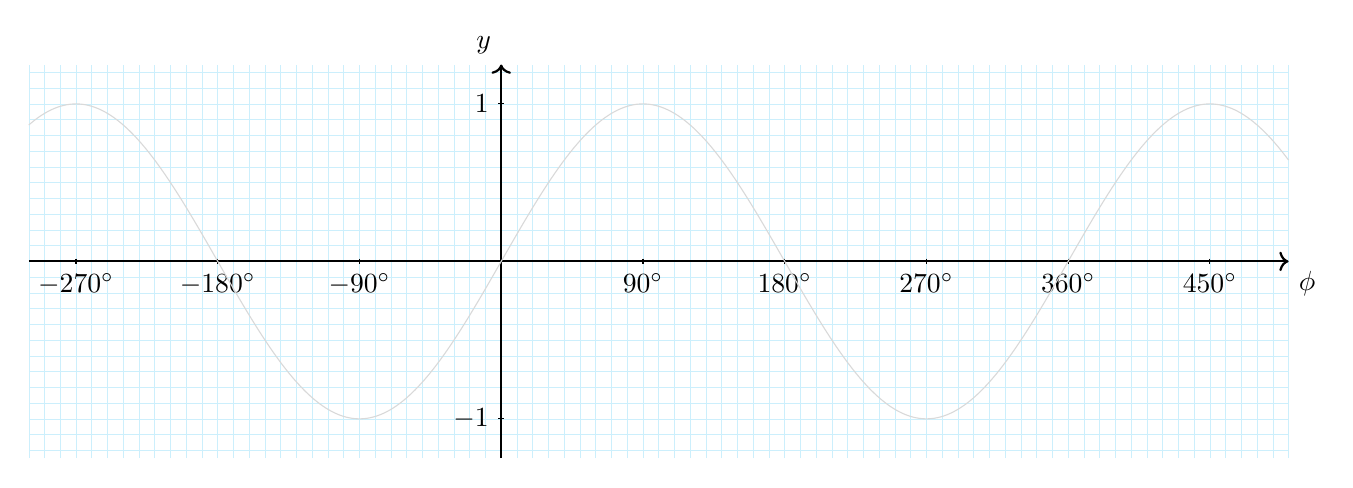
\begin{tikzpicture}
\draw[step = 0.2 cm, very thin, cyan!20] (-6, -2.5) grid ( 10, 2.5);
\draw[thick, ->] (-6,0) -- (10,0) node[anchor = north west] {$\phi$};
\draw[thick, ->] (0,-2.5) -- (0,2.5) node[anchor = south east] {$y$};

\foreach \x [evaluate=\x as \degree using int(\x*90)] in {-3,-2,-1,1,2,3,4,5}{ 
   \draw (\x *18mm, 1pt) -- (\x * 18mm, -1pt) node[anchor = north] {$\degree^\circ$};
   }
   
\foreach \y in {-1,1}
   \draw (1pt, \y *2cm) -- (-1pt, \y *2cm) node[anchor = east] {$\y$};

\draw[domain=-6:10,smooth,samples=200,variable=\x,gray!30] plot ({\x},{2*sin(\x*50)});
\end{tikzpicture}}%% END Definition

\newcommand{\trigsysDcos}{
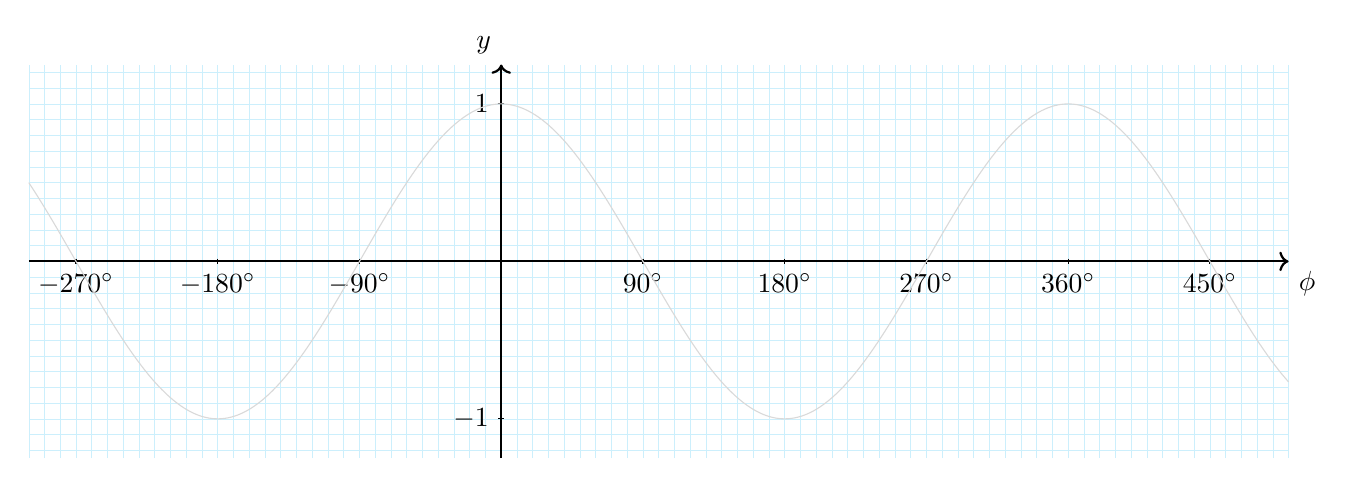
\begin{tikzpicture}
\draw[step = 0.2 cm, very thin, cyan!20] (-6, -2.5) grid ( 10, 2.5);
\draw[thick, ->] (-6,0) -- (10,0) node[anchor = north west] {$\phi$};
\draw[thick, ->] (0,-2.5) -- (0,2.5) node[anchor = south east] {$y$};

\foreach \x [evaluate=\x as \degree using int(\x*90)] in {-3,-2,-1,1,2,3,4,5}{ 
   \draw (\x *18mm, 1pt) -- (\x * 18mm, -1pt) node[anchor = north] {$\degree^\circ$};
   }
   
\foreach \y in {-1,1}
   \draw (1pt, \y *2cm) -- (-1pt, \y *2cm) node[anchor = east] {$\y$};

\draw[domain=-6:10,smooth,samples=200,variable=\x,gray!30] plot ({\x},{2*cos(\x*50)});
\end{tikzpicture}}%% END Definition


%%

\usepackage{bbwLayoutPageSty}


%%%%%%%%%%%%%%%  H E A D E R   &   F O O T E R %%%%%%%%%%%%%%%%%%%%
%% Headers
\fancyhf[HL]{\makebox{\includegraphics[width=30mm]{logos/bbw.pdf}}}%%
\fancyhf[HC]{\metaHeaderLine{}}%%
\fancyhf[FR]{\tiny{\shortAuthor{} (\today{})}}%%

\newcommand{\arbeitsblattHeader}{%%
  \begin{center}%%
    {\Large \fontfamily{qhv}\selectfont \arbeitsblattTitel{}}%%
\end{center}}%%

\renewcommand{\bbwAufgabenBlockID}{APot}


%%%%%%%%%%%%%%%%%%%%%%%%%%%%%%%%%%%%%%%%%%%%%%%%%%%%%%%%%%%%%%%%%%

\usepackage{amssymb} %% für \blacktriangleright
\renewcommand{\metaHeaderLine}{Potenzgesetze}
\renewcommand{\arbeitsblattTitel}{Version 1.1 Feb. 2024}

\begin{document}%%
\arbeitsblattHeader{}


%\newcounter{aufgabennummer}
%\setcounter{aufgabennummer}{1}

\newcommand\aufgabeML[3]{

\textbf{Aufgabe \arabic{bbwAufgabenNummerCounter}.} :\,\,
$${#2} = \TRAINER{{#3}}$$

\abplz{#1}

\stepcounter{bbwAufgabenNummerCounter}
}%% End command AufgabeML

{\huge{Vermischte Aufgaben zu Potenzgesetzen}}


\section{Zehnerpotenzen}

Berechnen Sie Zehnerpotenzen und vergleichen Sie:

\aufgabeML{2}{(-10)^4}{(-10)(-10)(-10)(-10) = 10\,000}
\aufgabeML{2}{-10^4}{-(10^4)=-(10\cdot{}10\cdot{}10\cdot{}10) = -10\,000}

\aufgabeML{2}{(-10)^5}{-100\,000}
\aufgabeML{2}{-10^7}{-10\,000\,000}
\aufgabeML{2}{(-10)^8}{+100\,000\,000}
\noTRAINER{\newpage}


\aufgabeML{2}{-(10^6)}{-1\,000\,000}

\aufgabeML{2}{0.1^1}{0.1}
\aufgabeML{2}{0.1^2}{0.01}
\aufgabeML{2}{-0.1^4}{-(0.1^4) = -0.0001}

\newpage

\textbf{Aufgabe \arabic{bbwAufgabenNummerCounter}. }:

Füllen Sie die Tabelle aus. Tipp: Welche Operation wird in den
hinteren drei Spalten konsequent von einer Zeile zur nächsten ausgeführt?

\begin{bbwFillInTabular}{|r|r|r|l|}\hline
Exponent       & Zehnerpotenz & Potenzwert & Name \\\hline
$4$            &  $10^4$           &  $10\,000$        & Zehntausend         \\\hline
$3$            &  \TRAINER{$10^3$} &  \TRAINER{$1000$} & \TRAINER{Tausend}   \\\hline
$2$            &  \TRAINER{$10^2$} &  \TRAINER{$100$}  & \TRAINER{Hundert}   \\\hline
$\TRAINER{1}$  &  \TRAINER{$10^1$} &  \TRAINER{$10$}   & \TRAINER{Zehn}      \\\hline
$\TRAINER{0}$  &  \TRAINER{$10^0$} &  \TRAINER{$1$}    & \TRAINER{Eins}      \\\hline
$\TRAINER{-1}$ &  \TRAINER{$10^{-1}$} &  \TRAINER{$0.1$}  & \TRAINER{Ein Zehntel}      \\\hline
$-2$           &  \TRAINER{$10^{-2}$} &  \TRAINER{$0.01$}	 & \TRAINER{Ein Hundertstel}      \\\hline
\end{bbwFillInTabular}
\stepcounter{bbwAufgabenNummerCounter}


Schreiben Sie ohne Klammern und ohne Bruchstrich:
\aufgabeML{2.4}{\frac1{10\,000}}{10^{-4}}

Fassen Sie die Zehnerpotenzen zusammen und schreiben Sie
wissenschaftlich (genau eine Ziffer vor dem Dezimalpunkt):

\aufgabeML{2.4}{9\cdot{}10^3 + 4.7 \cdot{}10^4}{5.6\cdot{} 10^4}
\aufgabeML{2.4}{2\cdot{}10^{-4} + 220.3 \cdot{} 10^{-5}}{2.403 \cdot{} 10^{-3}}



Multiplizieren Sie die Zehnerpotenzen (gleiche Basis):
\aufgabeML{2.8}{-0.1^4\cdot{} 0.1^5}{-0.1^{9} = -0.000\,000\,001}

\TRAINER{\newpage}
\textbf{Aufgabe \arabic{bbwAufgabenNummerCounter}.} :

Ein rotes Blutkörperchen hat ein Gewicht von $3\cdot{}10^{-11}$ g.
Beim Menschen liegt die Konzentration im Blut bei $4\,000$ bis $5\,900$ Stück pro Nanoliter.

\begin{bbwAufgabenBlock}
\item Geben Sie die Anzahl der roten Blutkörperchen je im Minimum und
im Maximum pro Liter Blut mit Hilfe von Zehnerpotenzen
an.\TRAINER{Minimal: $4000\cdot{}10^9 = 4\cdot{}10^{12}$, maximal:
$5.9\cdot{}10^{12}$}

\item Wie viele solcher Blutkörperchen hat ein Mensch, wenn wir von
einer Konzentration von 5\,000 Stück pro Nanoliter ausgehen und von
einer Blutmenge von 6 Litern? Wie heißt die Zahl in Worten?
\TRAINER{$6\cdot{} 5.0\cdot{}10^{}12 = 3.0 \cdot{} 10^{13}$ = 30
Billionen}

\item Wie groß ist die Masse aller roten Blutkörperchen einer Person,
wenn wir von 6 Liter Blut und 5\,000 roten Blutkörperchen pro
Nanoliter ausgehen?
\TRAINER{$3.0\cdot{}10^{13} \cdot{} 3\cdot{} 10^{-11} \text{ g } = 9\cdot{}10^2 \text{ g } = 900 \text{ g }$}
\end{bbwAufgabenBlock}

\TNTeop{}
%%%%%%%%%%%%%%%%%%%%%%%%%%%%%%%%%%%%%%%%%%%%%%%%%%%%%%%%%%%%%%%%%%%%%


\textbf{Aufgabe \arabic{bbwAufgabenNummerCounter}.} : Ölfilter

Eine Ölschicht auf einer ruhenden Wasseroberfläche sei ca. 0.08 mm
dick.

Ein Barrel (bbl.) fasst 159 Liter. Aus einem Öltanker fließen 277 bbl.
Öl aufs Meer.

\begin{bbwAufgabenBlock}
\item Geben Sie an, wie viel m$^3$ Öl ausgeflossen sind.

\TRAINER{227 bbw x 159 Liter pro bbl = 36093 Liter = 36.093 m$^3$.}

\item Wie groß in m$^2$ ist der dadurch entstehende Ölteppich ungefähr?
\TRAINER{36.093 [m$^3$] : 0.00008 [m] = 451162.5 m$^2$ $\approx$ 45 ha.}

\end{bbwAufgabenBlock}

\TNTeop{}

%%%%%%%%%%%%%%%%%%%%%%%%%%%%%%%%%%%%%%%%%%%%%%%%%%%%%%%%%%%%%%%%%%%%%%%%%%%%%%%%%%%%%%%%%%%%%%%%%%
\newpage
\section{Potenzgesetze}
Vereinfachen Sie / Fassen Sie zusammen:

\aufgabeML{2}{(-1)^{3}}{-1}
\aufgabeML{2}{(-1)^{4}}{1}
\aufgabeML{4}{ar^n - br^n}{(a-b)r^n}
\aufgabeML{6}{a^2(a-b)^n - b^2(a-b)^n}{(a^2-b^2)(a-b)^n = (a+b)(a-b)(a-b)^n = (a+b)(a-b)^{n+1}}
\noTRAINER{\newpage}

\aufgabeML{2}{-\left((-a)^3\right)^{10}}{-a^{30}}

\aufgabeML{2}{\left(-(-x^2)\right)^7}{x^{14}}

\aufgabeML{2}{\left(-x^3\right)^4}{x^{12}}
%%\platzFuerBerechnungenBisEndeSeite{}

\aufgabeML{2}{c^9 : c^4}{c^5}


\newpage
\subsection{gleiche Basis}
Multiplizieren Sie die Potenzen mit gleicher Basis:

\aufgabeML{4}{x^7\cdot{} x^{n+1}}{x^{n+8}}
\aufgabeML{4}{b^{k+3}\cdot{}b^{2k-1}}{b^{(k+3)+(2k-1)} = b^{3k+2}}
\aufgabeML{6}{-(s)^{8}\cdot{}s^7}{-s^{15}}
\noTRAINER{\newpage}


\aufgabeML{6}{(-s)^{8}\cdot{}s^7}{s^{15}}
\aufgabeML{6}{-2s^4\cdot{}s^3}{-2s^7}
\aufgabeML{6}{-(2s)^4\cdot{}s^3}{-8s^7}
\noTRAINER{\newpage}

\aufgabeML{6}{(-2s)^4\cdot{}s^3}{8s^7}
\aufgabeML{4}{(-r)^{5}\cdot{}(-r^6)}{+r^{11}}
\aufgabeML{4}{5\cdot{}2^{2n} + 4^n}{5\cdot{}4^n + 4^n = 6\cdot{}4^n}
\noTRAINER{\newpage}

\aufgabeML{6}{-b^{100}:b^{95}}{-b^5}
\aufgabeML{6}{x^{s+10} : x^{10}}{x^s}
\aufgabeML{6}{a^{5n-4} : a^{2n+3}}{a^{(5n-4)-(2n+3)} = b^{5n-4-2n-3} =
b^{3n-7}}
\noTRAINER{\newpage}


\aufgabeML{6}{(-a)^4:(-a^{10})}{-\frac{1}{a^6}}
\aufgabeML{6}{a\cdot{} a^{2x+3} : a^{1-x}}{a^{3x+3}}
\aufgabeML{6}{\left(\frac{x}{y}\right)^7:\left(\frac{-x}{y}\right)^3}{-\left(\frac{x}{y}\right)^4}
\noTRAINER{\newpage}


\aufgabeML{8}{\left(\left(\frac{-1}{2}\right)^3\right)^4}{\frac1{2^{12}}
= \frac1{4096}}
\aufgabeML{6}{(n^5)^{k-1}}{n^{5k-5}}
\noTRAINER{\newpage}


\aufgabeML{6}{(m^n)^n}{m^{(n^2)} = m^{n^2}}

%%%%%%%%%%%%%%%%%%%%%%%%%%%%%%%%%%%%%%%%%%%%%%%%%%%%%%%%%%%%%%%%%%%%%%%
\newpage
\subsection{Gleiche Exponenten}

\aufgabeML{4}{a^7 \cdot{} b^7}{(ab)^7}
\aufgabeML{4}{x^5 \cdot{} r^5}{\left(\frac{x}{r}\right)^5}
\aufgabeML{4}{(2x)^4\cdot{}y^4}{16(xy)^4}
\noTRAINER{\newpage}


\aufgabeML{4}{2a^5\cdot{}b^5}{2(ab)^5}
\aufgabeML{5.2}{1.25^{2s}\cdot{}8^{2s}}{10^{2s}}
\aufgabeML{8}{\left(\frac67\right)^n : \left(\frac37\right)^n}{2^n}
\noTRAINER{\newpage}


\aufgabeML{8}{16x^3 : (2y)^3}{16 \cdot{} (x:(2y)))^3 = 2\cdot{}2^3 \cdot{} \left(\frac{x}{2y}\right)^3  = 2 \cdot{} \left(\frac{x}{y}\right)^3}
\aufgabeML{6}{(-2p^3)^2 : (2q)^2}{\left((-2p^3) : (2q)\right)^2 =
(-p^3:q)^3}
\noTRAINER{\newpage}
\aufgabeML{6}{(-2a)^3: (-2b)^3}{\left(\frac{a}{b}\right)^3}




\newpage
\subsection{Erste Exponentialgleichungen}
Bringen Sie beide Seiten auf dieselbe Basis und Lösen Sie durch
Exponentenvergleich:

\aufgabeML{6}{7^{19} \cdot{} 7^3 = 7^x}{19 + 3 = x \Longrightarrow x = 22}
\aufgabeML{6}{\left(a^{10}\right)^x = a^{150}}{10x = 150 \Longrightarrow x = 15}
\aufgabeML{6}{\left(a^x\right)^3 \cdot{} a^5= \left(a^2\right)^x \cdot{}a^7}{3x+5=2x+7\Longrightarrow x = 2}


\newpage
\section{negative Exponenten und die Null}
\subsection{Zehnerpotenzen}
\aufgabeML{2}{10^{-4}}{0.0001}
\aufgabeML{2}{(-10)^{-3}}{-0.001}
\aufgabeML{2}{0.01^{-2}}{10\,000}
\aufgabeML{2}{(-0.1)^{-2}}{100}

\newpage
\subsection{Mit Variablen}

Geben Sie die Lösung für verschiedene $n \in \mathbb{N}$ an:
\aufgabeML{6}{(-1)^{-(2n+1)}}{-1 \text{ für alle } n}

\aufgabeML{6}{\frac{-3}{-x^{-4}}}{3x^4}
\noTRAINER{\newpage}

Vereinfachen Sie: 
\aufgabeML{6}{\frac{a^2}{a^3}}{\frac{1}{a}=a^{-1}}

\aufgabeML{6}{-\left(-(-a)^2\right)^0}{-1}
\noTRAINER{\newpage}


\aufgabeML{6}{a^5\cdot{}a^{-2}\cdot{}a^0\cdot{}a^{7}\cdot{}a\cdot{}a^{-4}}{a^{7}}

\aufgabeML{4}{\left(x^{-1}\right)^{-1}}{x}

\aufgabeML{4}{\left( \left( \left(  \left(   \frac37b^{-7} \right)^{14}  \right)^0 \right)^{-3}
\right)^8}{1}
\noTRAINER{\newpage}


\aufgabeML{6}{(ab)^{-4} \cdot{} \left(\frac{c}{d}\right)^{-4}}{\left(\frac{abc}{d}\right)^{-4}}

\aufgabeML{6}{(ab)^{-n} : \left(\frac{a}{b}\right)^{-n}}{\left(ab
: \frac{a}{b}\right)^{-n} = \left(ab \cdot \frac{b}{a} \right)^{-n}
= \left(b^2\right)^{-n} = b^{-2n}}
\noTRAINER{\newpage}

\aufgabeML{6}{-\left( -a^3\cdot{} (-a)^2 \right)^{-4}}{\frac{-1}{a^{20}} = -a^{-20}}

\aufgabeML{6}{(-b)^{-6} \cdot (-b^8)}{-b^2}

\aufgabeML{6}{\left(-(a^{-1})^{-2}\right)^6}{a^{12}}\noTRAINER{\newpage}

\aufgabeML{6}{-\left((a^3)\cdot{}a^{-1}\right)^2}{-a^4}

Schreiben Sie ohne negative Exponenten:

\aufgabeML{4}{2\cdot{}x^{-3}}{\frac{2}{x^3}}

\aufgabeML{4}{ab^{-5}}{\frac{a}{b^5}=a\cdot{}\frac{1}{b^5}}
\noTRAINER{\newpage}
\aufgabeML{6}{\frac{1}{81}\cdot{}c^{-2}\cdot{}a^{-3}\cdot{}c^2\cdot{} a^3 \cdot 3^4}{1}

\aufgabeML{6}{\frac1{125}\cdot{}b^{3}\cdot{}b^{0}\cdot{}b^6\cdot{} b^{-4} \cdot 5^2}{\frac1{5}b^5}
%%\platzFuerBerechnungenBisEndeSeite{}

\newpage
\section{negative Exponenten mit Brüchen}
\aufgabeML{6}{\frac{6\cdot{} a^3 \cdot{} b^7 \cdot{} 3}{(ab)^4\cdot 9 \cdot a^{-1}}}{2b^3}

\aufgabeML{6}{\left(\frac{a^2 b^{-3} c^3}{a\cdot b}\right)^{-3}\cdot \left(\frac{c^5}{ab}\right)^2}{\frac{b^{10}c}{a^5}}\noTRAINER{\newpage}

\aufgabeML{6}{\left(\frac{ab^{-2}c^3}{a^{-2}\cdot{}b}\right)^{-2} \cdot{} \left(\frac{a^3\cdot{} c^{2}}{b^2} \right)^3}{a^3}


\aufgabeML{6}{\left(\frac{a^3 \cdot{}c^{-1}}{b^{-2}}\right)^{-4} \cdot \left( \frac{a^4\cdot{}b^3}{c^{-2}} \right)^3}{bc^{10}}\noTRAINER{\newpage}

\aufgabeML{6}{\frac{a^{-5}\cdot{} (-a)^3}{a^7} : \frac{a^{-10}}{a^4} }{-a^5}

\aufgabeML{6}{\frac{ab\cdot{}b^{-2}\cdot{}b^4\cdot{}b^{-3}}{b^3\cdot{}a\cdot{}b^{-4} \cdot{} b}}{1}\noTRAINER{\newpage}


\aufgabeML{6}{\left(\frac{3x^{-2}y^2}{4x^{-4}\cdot{}y^3}\right)^{-2} : \left(\frac{2x^{-1}}{3xy^{-2}}\right)^3}{\frac{6x^2}{y^4}}

\aufgabeML{6}{4^k\cdot{} \left(\frac{1}{2}\right)^k \cdot{} \left(\frac{1}{3}\right)^{-k}}{6^k}\noTRAINER{\newpage}

\aufgabeML{6}{\frac{a^{-2}}{a^{-3}}}{a}

\aufgabeML{6}{\left(\frac{a^4\cdot{}b^{-2}\cdot{}c}{a^2\cdot{}c^{-3}}\right)^{-2} \cdot \left(\frac{c^2\cdot{}b}{a^{-1}}\right)^4}{b^8}\noTRAINER{\newpage}


\aufgabeML{6}{\left(\frac{3a^{-1}\cdot{} b^2}{2ac^{-1}}\right)^{-2} \cdot{} \frac{\left(3\cdot{}b^2\right)^2\cdot{}c^2}{4}}{a^4}

\aufgabeML{6}{a^{-1}\cdot{} a^{-2} : a^{-3} \cdot{} a^7}{a^7}\noTRAINER{\newpage}
\newpage
Kürzen Sie:

\aufgabeML{6}{\frac{a^{15} - a^{10}}{a^5}}{a^{10} - a^5}
\aufgabeML{6}{\frac{b^6 + b^9}{b^7 - b^{11}}}{\frac{1+b^3}{b - b^5}}

\newpage
\subsection{vermischte Exponentialgleichungen}
Bringen Sie beide Seiten auf dieselbe Basis und Lösen Sie durch
Exponentenvergleich:

\aufgabeML{6}{(a^3)^x = \frac{a^{2x}}{a^{-2}}}{3x = 2x - (-2) \Longrightarrow 3x = 2x+2 \Longrightarrow x=2}
\aufgabeML{6}{2^x = 4^{-4}}{2^x = 2^{-8} \Longrightarrow x=-8}
\noTRAINER{\newpage}

\aufgabeML{6}{(3^x)^6 = \frac1{81}}{3^{6x = 3^{-4}} \Longrightarrow 6x
= -4 \Longrightarrow x = -4 : 6 = \frac{-2}{3}}

Das folgende ist keine Exponentialgleichung, kann aber gelöst werden,
indem auf beiden Seiten der Gleichung der selbe Exponent erzwungen
wird:

\aufgabeML{6}{x^3=125^{-1}}{x^3 = \frac1{125} = \frac1{5^3}
= \left(\frac15\right)^3 \Longrightarrow x = \frac15}

%%%%%%%%%%%%%%%%%%%%%%%%%%%%%%%%%%%%%%%%%%%%%%%%%%%%%%%%%%%%%%%%%%%%%%
\newpage
\section{Wurzeln}

\aufgabeML{4}{\left(\sqrt[2]{x}\right)^2}{x}
\aufgabeML{6}{\sqrt[3]{b^3}}{b}
\aufgabeML{4}{\sqrt[6]{0.000001}}{0.1}\noTRAINER{\newpage}


\aufgabeML{4}{\sqrt[3]{\sqrt[4]{\sqrt{2}}}}{\sqrt[24]{2}}

\aufgabeML{2}{\sqrt{a^2}}{|a|}


\aufgabeML{6}{\sqrt[3]{z^9}}{z^3}\noTRAINER{\newpage}

\aufgabeML{6}{\sqrt[5]{b^{10}r^5}}{b^2r}

\aufgabeML{6}{\sqrt[4]{r^8n^{12}}}{r^2|n|^3}

\aufgabeML{6}{\sqrt[5]{m^4\cdot{m}}}{m}\noTRAINER{\newpage}

\aufgabeML{6}{\sqrt{m^2+m^2 + m^2}}{\sqrt{3}\cdot{}m}

\aufgabeML{6}{\sqrt{\sqrt[2]{x^4}}}{x}

\aufgabeML{6}{\frac{\sqrt[3]{a^7}}{\sqrt[3]{a}}}{a^2}\noTRAINER{\newpage}

\aufgabeML{6}{\sqrt[8]{r^{24}}}{r^3}
\noTRAINER{\newpage}

Und als Überleitung ins nächste Thema:

\aufgabeML{6}{\sqrt[6]{v^3}}{v^{\frac12} = \sqrt{v}}

\newpage
\section{Rationale Exponenten}

\aufgabeML{4}{\sqrt{\sqrt[3]{10}\cdot{}\sqrt[4]{10}}}{\sqrt[24]{10^7}}

\aufgabeML{6}{a^4\cdot{}a^{\frac{1}{4}}\cdot a^5\cdot a^{\frac{-1}{5}}}{a^\frac{181}{20}}

\aufgabeML{6}{\sqrt[4]{a^3}}{a^{\frac{3}{4}}}\noTRAINER{\newpage}

\aufgabeML{6}{\sqrt[3]{r^{\frac{3}{4}}}}{\sqrt[4]{r} = r^{\frac{1}{4}}}

\aufgabeML{6}{\sqrt{b^\frac12}}{\sqrt[4]b = b^\frac14}\noTRAINER{\newpage}

\aufgabeML{6}{\sqrt{a^\frac{1}{2}} \cdot \sqrt[4]{a\cdot{} \sqrt[5]{a^{10}}}}{a}

\aufgabeML{6}{\sqrt{x^{10}} \cdot \sqrt[4]{x^3} \cdot x^{\frac{1}{4}}}{x^6}\noTRAINER{\newpage}

\aufgabeML{6}{\sqrt[3]{a} \cdot \sqrt{a^3 \cdot \sqrt[3]{a}}}{a^2}

\aufgabeML{6}{\sqrt[3]{a^2} \cdot \sqrt[4]{a^3 \cdot \sqrt[3]{a}}}{a^{\frac{9}{6}} = \sqrt[6]{a^9} = a^\frac32 = \sqrt{a^3}}\noTRAINER{\newpage}

\aufgabeML{6}{\sqrt[3]{b\cdot \sqrt{b^3\cdot \sqrt[3]b}}}{\sqrt[9]{b^8}}

\aufgabeML{6}{\sqrt[4]{b\cdot{} \sqrt[3]{b^2\cdot \sqrt{b}}}}{b^\frac{11}{24} = \sqrt[24]{b^{11}}}\noTRAINER{\newpage}

\aufgabeML{6}{3a\cdot \sqrt[3]{9a^2}}{\sqrt[3]{3^5 a^5} = \left(3a\right)^\frac53}

\aufgabeML{6}{\sqrt{x} \cdot \sqrt[3]{x^4} \cdot \sqrt[6]{x^3}}{x^\frac73 = \sqrt[3]{x^7}}\noTRAINER{\newpage}

\aufgabeML{6}{\sqrt{a^3}\cdot \sqrt[3]{a^2}}{a^\frac{13}{6} = \sqrt[6]{a^{13}}}

\aufgabeML{6}{\sqrt{a^2 \sqrt{a}}}{a^\frac54 = \sqrt[4]{a^5}}\noTRAINER{\newpage}

\aufgabeML{6}{\sqrt{a^{-2}}}{\frac{1}{a} = a^{-1}}

\aufgabeML{6}{\sqrt[3]{a^2 \cdot b \cdot \sqrt{a\cdot b^{-1}}}}{a^\frac56 \cdot b^\frac16 = \sqrt[6]{a^5\cdot b}}\noTRAINER{\newpage}

\aufgabeML{6}{\sqrt{x^3} \cdot \left(\sqrt{x}\right)^{-3}}{1}

\aufgabeML{6}{\frac{\sqrt{a^3}}{\sqrt{a^{-1}}}}{a^2}\noTRAINER{\newpage}

\aufgabeML{6}{\left(\frac{1}{a}\right)^{-\frac14}}{\sqrt[4]a = a^\frac14}

\aufgabeML{6}{\frac{a^4}{\sqrt{a}}}{\sqrt{a^7} = (\sqrt{a})^7 = a^\frac72}\noTRAINER{\newpage}

\aufgabeML{6}{\frac{\sqrt[3]{a^2}}{\sqrt{a}}}{a^{\frac16} = \sqrt[6]{a}}

\aufgabeML{6}{\frac{-\sqrt{a^3}}{-\left(\sqrt{a}\right)^3}}{1}\noTRAINER{\newpage}

\aufgabeML{6}{\frac{\sqrt[3]{a^{13}}}{a^4}}{a^{\frac13} = \sqrt[3]{a}}


\aufgabeML{6}{\sqrt[3]{26\cdot{} \sqrt[4]{a^3} + \sqrt[8]{a^6}}}{3\cdot{}\sqrt[4]{a}}
%%\platzFuerBerechnungenBisEndeSeite{}

\end{document}
